\documentclass[twoside]{article}
\usepackage{amsmath}
\usepackage{amssymb}
\usepackage{amsthm}
\usepackage{calc}
\usepackage{capt-of}
\usepackage{caption}
\usepackage[strict]{changepage}
\usepackage{chngcntr}
\usepackage[americanvoltage,siunitx]{circuitikz}
\usepackage{color,colortbl}
\usepackage{etoolbox}
\usepackage{fancyhdr}
\usepackage[T1]{fontenc}
\usepackage{gensymb}
\usepackage[margin=1in]{geometry}
\usepackage{graphicx}
\usepackage{hyperref}
\usepackage{import}
\usepackage{indentfirst}
\usepackage{mathptmx}
\usepackage{mathrsfs}
\usepackage{multicol}
\usepackage{multirow}
\usepackage{needspace}
\usepackage{pgfplots}
\usepackage{pgfplotstable}
\usepackage{setspace}
\usepackage{siunitx}
\usepackage{tabu}
\usepackage{tabularx}
\usepackage{tikz}
\usepackage{xspace}

\patchcmd{\thebibliography}{\section*{\refname}}{\vspace{-1em}}{}{}

\captionsetup{labelformat=empty,labelsep=none}
\usepgfplotslibrary{external}
\usetikzlibrary{positioning,matrix,shapes,chains,arrows}
\tikzexternalize[prefix=precompiled_figures/]

\newcommand\svgsize[2]{\def\svgwidth{#2}
{\centering\input{#1.pdf_tex}}}
\newcommand\svgc[1]{\svgsize{#1}{\columnwidth}}
\newcommand\svgl[1]{\svgsize{#1}{1em}}
\newcommand\diagrams[0]{\renewcommand\svgsize[2]{\def\svgwidth{##2}
{\centering\input{diagrams/##1.pdf_tex}}}}

\newcommand\pdf[1]{\noindent\includegraphics[width=\columnwidth]{#1.pdf}}
\newcommand\pdfex[1]{\pdf{#1}

\pdf{#1ex}}
\newcommand\pdfmsg[1]{\noindent\begin{minipage}{\columnwidth}\pdf{#1msg}

\pdf{#1}\end{minipage}}
\newcommand\pdfmsgex[1]{\pdfmsg{#1}

\pdf{#1ex}}
\newcommand\code[0]{\renewcommand\pdf[1]{\noindent
\includegraphics[width=\columnwidth]{code/##1.pdf}}}

% Indent
\setlength{\parindent}{0.3in}

\newcounter{paperthmamount}
\newcommand\theorems[0]{
\theoremstyle{remark}
\newtheorem{claim}[subsection]{Claim}
\theoremstyle{plain}
\newtheorem{conjecture}[subsection]{Conjecture}
\theoremstyle{plain}
\newtheorem{corollary}[subsection]{Corollary}
\theoremstyle{definition}
\newtheorem{definition}[subsection]{Definition}
\theoremstyle{plain}
\newtheorem{lemma}[subsection]{Lemma}
\theoremstyle{remark}
\newtheorem{proposition}[subsection]{Proposition}
\theoremstyle{remark}
\newtheorem{remark}[subsection]{Remark}
\theoremstyle{plain}
\newtheorem{theorem}[subsection]{Theorem}
\theoremstyle{definition}
\newtheorem{question}[subsection]{Question}
\newcommand\paperclm[2]
{\begin{claim}\global\expandafter\edef
\csname clm##1\endcsname{Claim \thesubsection\noexpand\xspace}
##2\end{claim}}
\newcommand\papercnj[2]
{\begin{conjecture}\global\expandafter\edef
\csname cnj##1\endcsname{Conjecture \thesubsection\noexpand\xspace}
##2\end{conjecture}}
\newcommand\papercor[2]
{\begin{corollary}\global\expandafter\edef
\csname cor##1\endcsname{Corollary \thesubsection\noexpand\xspace}
##2\end{corollary}}
\newcommand\paperdef[2]
{\begin{definition}\global\expandafter\edef
\csname def##1\endcsname{Definition \thesubsection\noexpand\xspace}
##2\end{definition}}
\newcommand\paperlem[2]
{\begin{lemma}\global\expandafter\edef
\csname lem##1\endcsname{Lemma \thesubsection\noexpand\xspace}
##2\end{lemma}}
\newcommand\paperprp[2]
{\begin{proposition}\global\expandafter\edef
\csname prp##1\endcsname{Proposition \thesubsection\noexpand\xspace}
##2\end{proposition}}
\newcommand\paperqtn[2]
{\begin{question}\global\expandafter\edef
\csname qtn##1\endcsname{Question \thesubsection\noexpand\xspace}
##2\end{question}}
\newcommand\paperrem[2]
{\begin{remark}\global\expandafter\edef
\csname rem##1\endcsname{Remark \thesubsection\noexpand\xspace}
##2\end{remark}}
\newcommand\paperthm[2]
{\begin{theorem}\global\expandafter\edef
\csname thm##1\endcsname{Theorem \thesubsection\noexpand\xspace}
##2\end{theorem}}}
\newcommand\subtheorems[0]{\stepcounter{paperthmamount}
\theoremstyle{remark}
\newtheorem{claim}[subsubsection]{Claim}
\theoremstyle{plain}
\newtheorem{conjecture}[subsubsection]{Conjecture}
\theoremstyle{plain}
\newtheorem{corollary}[subsubsection]{Corollary}
\theoremstyle{definition}
\newtheorem{definition}[subsubsection]{Definition}
\theoremstyle{plain}
\newtheorem{lemma}[subsubsection]{Lemma}
\theoremstyle{remark}
\newtheorem{proposition}[subsubsection]{Proposition}
\theoremstyle{remark}
\newtheorem{remark}[subsubsection]{Remark}
\theoremstyle{plain}
\newtheorem{theorem}[subsubsection]{Theorem}
\theoremstyle{definition}
\newtheorem{question}[subsubsection]{Question}
\newcommand\paperclm[2]
{\begin{claim}\global\expandafter\edef
\csname clm##1\endcsname{Claim \thesubsubsection\noexpand\xspace}
##2\end{claim}}
\newcommand\papercnj[2]
{\begin{conjecture}\global\expandafter\edef
\csname cnj##1\endcsname{Conjecture \thesubsubsection\noexpand\xspace}
##2\end{conjecture}}
\newcommand\papercor[2]
{\begin{corollary}\global\expandafter\edef
\csname cor##1\endcsname{Corollary \thesubsubsection\noexpand\xspace}
##2\end{corollary}}
\newcommand\paperdef[2]
{\begin{definition}\global\expandafter\edef
\csname def##1\endcsname{Definition \thesubsubsection\noexpand\xspace}
##2\end{definition}}
\newcommand\paperlem[2]
{\begin{lemma}\global\expandafter\edef
\csname lem##1\endcsname{Lemma \thesubsubsection\noexpand\xspace}
##2\end{lemma}}
\newcommand\paperprp[2]
{\begin{proposition}\global\expandafter\edef
\csname prp##1\endcsname{Proposition \thesubsubsection\noexpand\xspace}
##2\end{proposition}}
\newcommand\paperqtn[2]
{\begin{question}\global\expandafter\edef
\csname qtn##1\endcsname{Question \thesubsubsection\noexpand\xspace}
##2\end{question}}
\newcommand\paperrem[2]
{\begin{remark}\global\expandafter\edef
\csname rem##1\endcsname{Remark \thesubsubsection\noexpand\xspace}
##2\end{remark}}
\newcommand\paperthm[2]
{\begin{theorem}\global\expandafter\edef
\csname thm##1\endcsname{Theorem \thesubsubsection\noexpand\xspace}
##2\end{theorem}}}

% Title section
\pagestyle{fancy}
\thispagestyle{empty}
\renewcommand{\headrulewidth}{0pt}
\newcommand\papertitle[1]
{{\centering\fontsize{20pt}{20pt}\textsc{#1}\\\mbox{}\\}
\fancyhead[OC]{\fontsize{12pt}{12pt}\selectfont\textit{#1}}}
\newcounter{people}
\newcommand\paperauthtext[3]{{\centering\fontsize{12pt}{12pt}\selectfont
\textsc{#1}\\[-0.1em]{\fontsize{9pt}{9pt}\selectfont\textit{\ifx&#2&
\vspace{-1em}\else#2\fi}}\\\mbox{}\\
\fancyhead[EC]{\fontsize{12pt}{12pt}\selectfont\textit{#3}}}}
\newcommand\paperauth[2]{{\stepcounter{people}
\ifnum\value{people}=1
{\paperauthtext{#1}{#2}{#1}
\global\def\auth{#1\xspace}}
\else\ifnum\value{people}=2
{\paperauthtext{#1}{#2}{\auth and #1}}
\else{\paperauthtext{#1}{#2}{\auth et al}}\fi\fi}}
\newcommand\physics[0]{
\renewcommand\paperauthtext[4]{{\centering\fontsize{12pt}{12pt}\selectfont
\textsc{##1. ##2}\\[-0.1em]{\fontsize{9pt}{9pt}\selectfont\textit{\ifx&##3&
\vspace{-1em}\else##3\fi}}\\\mbox{}\\
\fancyhead[EC]{\fontsize{12pt}{12pt}\selectfont\textit{##4}}}}
\renewcommand\paperauth[3]{{\stepcounter{people}
\ifnum\value{people}=1
{\paperauthtext{##1}{##2}{##3}{##1. ##2}
\global\def\auth{##2\xspace}}
\else\ifnum\value{people}=2
{\paperauthtext{##1}{##2}{##3}{\auth and ##2}}
\else{\paperauthtext{##1}{##2}{##3}{\auth et al}}\fi\fi}}}
\newcommand\paperdate[1]{{\centering\fontsize{9pt}{9pt}\selectfont\text{
(Received #1)}\\[2em]}}

% Page header
\newcommand{\paperhead}[1]{\fancyhead[EC]{\fontsize{12pt}{12pt}\selectfont
\textit{#1}}}
\fancyhead[RO, EL]{\fontsize{12pt}{12pt}\selectfont\thepage}
\fancyhead[RE, OL]{}
\cfoot{}

\makeatletter
\newenvironment{paperadjustwidth}[2]{
  \begin{list}{}{
    \setlength\partopsep\z@
    \setlength\topsep\z@
    \setlength\listparindent\parindent
    \setlength\parsep\parskip
    \@ifmtarg{#1}{\setlength{\leftmargin}{\z@}}
                 {\setlength{\leftmargin}{#1}}
    \@ifmtarg{#2}{\setlength{\rightmargin}{\z@}}
                 {\setlength{\rightmargin}{#2}}
    }
    \item[]}{\end{list}}
\makeatother

%Figure counter
\newcounter{paperfigurecounter}
\newcommand{\papercap}[2]{\bgroup\stepcounter{paperfigurecounter}
\captionof{figure}{\fontsize{9pt}{9pt}\selectfont
\hspace{0.3in}Fig.~\arabic{paperfigurecounter}.\quad#2}
\egroup\expandafter\edef
\csname fig#1\endcsname{Fig.~\arabic{paperfigurecounter}\noexpand\xspace}}

\newcommand\paperfig[3]{\noindent\begin{minipage}{\columnwidth}
#2\papercap{#1}{#3}\end{minipage}\expandafter\edef
\csname fig#1\endcsname{Fig.~\arabic{paperfigurecounter}\noexpand\xspace}}
\newcommand\papersvg[3]{\paperfig{#1}{\svgc{#2}}{#3}}

% Abstract environment
\newenvironment{paperabs}
{\begin{paperadjustwidth}{0.5in}{0.5in}\bgroup\fontsize{9pt}{9pt}\selectfont
\hspace{0.5in}}
{\egroup\end{paperadjustwidth}}

% Paper environment
\setlength\columnsep{0.5in}
\newenvironment{paper}
{\begin{multicols*}{2}\bgroup\fontsize{12pt}{12pt}\selectfont}
{\egroup\end{multicols*}}
\newcommand{\singlecolumn}[0]{
\renewcommand\paperfig[3]{\noindent
\makebox[\textwidth][c]{\begin{minipage}{5.5in}
\noindent\makebox[\textwidth][c]{\begin{minipage}{3in}##2\end{minipage}}
\papercap{##1}{##3}\end{minipage}}\expandafter\edef
\csname fig##1\endcsname{Fig.~\arabic{paperfigurecounter}\noexpand\xspace}}
\renewenvironment{paper}{\bgroup\fontsize{12pt}{12pt}\selectfont}
{\egroup}}

%Sources
\newsavebox{\sourcebox}
\newcommand{\papersource}[1]{
\vspace{-2em}
\text{}\\*
\fontsize{9pt}{9pt}\selectfont
\noindent\renewcommand{\labelenumi}{}
\savebox{\sourcebox}{\parbox{3in}{\begin{enumerate}
\setlength{\leftmargini}{-1ex}
\setlength{\leftmargin}{-1ex}
\setlength{\labelwidth}{0pt}
\setlength{\labelsep}{0pt}
\setlength{\listparindent}{0pt}
\item\textit{\hspace{-0.35in}#1}
\end{enumerate}}}
\usebox{\sourcebox}
}

%Section headers
\newcounter{paperseccounter}
\newcounter{papersubseccounter}[paperseccounter]
\newcommand\papersec[1]{\needspace{1in}
\stepcounter{paperseccounter}
\stepcounter{section}
\begin{center}\Roman{paperseccounter} \textsc{#1}\end{center}}
\newcommand\papersubsec[1]{\needspace{1in}
\stepcounter{papersubseccounter}
\addtocounter{subsection}{\thepaperthmamount}
\setcounter{subsubsection}{0}
{\begin{center}
\Roman{section}.\Roman{papersubseccounter}
\textsc{#1}\\[0.5em]\end{center}}}

%equation
\newcounter{papereqcounter}
\newcommand\papereq[3]{{
\stepcounter{papereqcounter}
\mbox{}\vspace{-0.75em}
\begin{equation*}
#2
\tag*{\fontsize{12pt}{12pt}\selectfont
$\begin{array}{r}
\cr{\text{(\arabic{papereqcounter})}}
\cr{\fontsize{9pt}{9pt}\selectfont\textit{\ifx\\#3\\~\else(\fi#3\ifx\\#3\\~
\else)\fi}}
\end{array}$}
\end{equation*}

}
\expandafter\edef\csname eq#1\endcsname{(\arabic{papereqcounter})\noexpand
\xspace}}

% Where
\newcommand{\papervar}[3]
{&$#1$ & #2 \ifx\\#3\\~\else($\smash{\text{\si{\fi
#3\ifx\\#3\\~\else}}}$)\fi\\}
\newenvironment{paperwhere}
{\begin{minipage}{\columnwidth}
\bgroup\fontsize{9pt}{9pt}\selectfont Where:\vspace{2pt}\\\begin{tabular}
{rr@{ = }p{\linewidth}}}
{\end{tabular}\egroup\end{minipage}\vspace{5pt}}

% Tables
\definecolor{LineGray}{gray}{0.5}
\newtabulinestyle{outer=2.25pt LineGray}
\newtabulinestyle{inner=0.75pt LineGray}
\tabulinesep=1.5pt

\newcommand{\paperiline}[0]{\tabucline[inner]{-}}
\newcommand{\paperoline}[0]{\tabucline[outer]{-}}

% Index column type
\newcolumntype{I}{X[-5,c]}
% Column type with uncertainty
\newcolumntype{U}{@{}X[-5,r]@{$\pm$}X[-5,l]@{}}
% Column type without uncertainty
\newcolumntype{C}{@{}X[-5,c]@{}}

\newcounter{papertableindexcounter}
\newcommand{\papertableindexheader}[0]{\multirow{2}{*}{\textsc{Index}}}
\newcommand{\papertableindex}[0]{\stepcounter{papertableindexcounter}
\arabic{papertableindexcounter}}
\newcommand{\papertableuheadersymbol}[1]{&\multicolumn{2}{c|[inner]}{$#1$}}
\newcommand{\papertableuheadersymbole}[1]{&\multicolumn{2}{c|[outer]}{$#1$}}
\newcommand{\papertableuheaderunit}[1]{&\multicolumn{2}{c|[inner]}{(#1)}}
\newcommand{\papertableuheaderunite}[1]{&\multicolumn{2}{c|[outer]}{(#1)}}
\newcommand{\papertablecheadersymbol}[1]{&$#1$}
\newcommand{\papertablecheaderunit}[2]{&($\pm$#1 #2)}

% Value in table with uncertainty.
\newcommand{\papertableuval}[2]{& #1 & #2}
% Value in table without uncertainty.
\newcommand{\papertablecval}[1]{& #1}

\newenvironment{papertable}[1]
{\setcounter{papertableindexcounter}{0} 
\begin{tabu} to \linewidth {#1}}
{\end{tabu}\vspace{12pt}}

\newcommand{\paperaxis}[9]
{title=#1,
axis x line = bottom,
xmin=#4,xmax=#6,
axis y line = left,
ymin=#5,ymax=#7,
height = 180pt,
grid=both,
x axis line style=-,
y axis line style=-,
x tick label style={
/pgf/number format/.cd,
fixed,
fixed zerofill,
precision=#8,
/tikz/.cd},
y tick label style={
/pgf/number format/.cd,
fixed,
fixed zerofill,
precision=#9,
/tikz/.cd}}
\newcommand{\paperaxisxlabel}[2]{
xlabel=\fontsize{10pt}{10pt}\selectfont#1$(#2)\rightarrow$}
\newcommand{\paperaxisylabel}[2]{
ylabel=\fontsize{10pt}{10pt}\selectfont#1$(#2)\rightarrow$}
\newcommand{\papergraphoutline}[4]{
\addplot [mark=none,line width=0.75pt] coordinates {
(#1,#2)
(#1,#4)
(#3,#4)
(#3,#2)
(#1,#2)};}

\newenvironment{papergraph}{
\begin{tikzpicture}
\begin{axis}}
{\end{axis}
\end{tikzpicture}}

\newcommand{\comment}[1]{}

\newcommand{\abs}[1]{\left\lvert#1\right\rvert}
\newcommand{\oo}[0]{\infty}
\newcommand{\sigmaSum}[3]{\sum\limits_{#1}^{#2} #3}
\newcommand{\limto}[3]{\lim\limits_{#1\rightarrow#2}#3}
\renewcommand{\d}[0]{\mathrm{d}}
\newcommand{\cross}[0]{\times}
\newcommand{\lp}{\left(}
\newcommand{\rp}{\right)}
\newcommand\pars[1]{\lp#1\rp}
\newcommand\sqbrack[1]{\left[#1\right]}
\newcommand\R{\mathbb{R}}
\newcommand\di{\partial}
\newcommand\x{\times}
\newcommand\del{\nabla}


\physics
\begin{document}
\papertitle{Analysis of a Thermo-Electric Cooler}
\paperauth{A}{Khesin}{1002442029}
\paperauth{P}{Zavyalova}{1002345036}
\paperdate{February 12, 2018, Completed February 6, 2018}
\begin{paperabs}
	
	This experiment investigated the properties of thermoelectric cooling. This
process is based on the Peltier and Seeback effects to use energy to pump heat.
This experiment measured various properties of the thermoelectric cooler.
The thermal conductance between the two reservoirs, $K_d$, was found to be $(0.59\pm.06)\si{\watt\per\kelvin}$.
The thermal conductance between the output heat sink and the ambient, $K_{hs}$, air was found to be $(7.1\pm.9)\si{\watt\per\kelvin}$.
The Seebeck coefficient for the system, $S_d$, was determined to be $(11.6\pm.1)\si{\milli\volt\per\kelvin}$.
The internal resistance of the thermoelectric cooler, $R_d$, was determined to be $(0.19\pm.01)\si{\ohm}$.
The lowest achievable temperature at the thermal reservoir with no heat input was determined to be $(-9.1\pm.2)\si{\kelvin}$.
The optimum drive current for the system was determined to be $(17.0\pm.9)\si{\ampere}$.
The lowest achievable temperature with the optimum input current was determined to be $(-18.4\pm.3)\si{\celsius}$.
	
\end{paperabs}

\begin{paper}
	
\papersec{Introduction}
	
	A thermo-electric cooler (TEC) is a device that exploits Peltier and Seebeck effects to act as a solid-state heat pump. Composed of a set of metal-to-semiconductor thermocouple junctions, the TEC is capable of transferring heat from a cold environment to a warmer one, essentially acting as a reverse heat engine. 
	
	The Seebeck effect refers to the process of a temperature difference being converted into electricity. Given a circular loop composed of two different metals, it is evident that when maintained at the same temperature, the wires have different electron densities. As electrons move in the loop to correct the electron imbalance, net electric fields are created at the junctions. Further, introducing a temperature difference by keeping one junction at a constant temperature and increasing the temperature of the other gives electrons more kinetic energy and thus resulting in charge imbalances being corrected faster at the warmer junction. A net electric field is created in the loop; an electric potential difference and a current flow are established in the loop.
	
	The inverse of the Seebeck effect is referred to as the Peltier effect. As electric current passes through a loop made of two different junctions, a temperature difference between the two junctions is established. The junction where electron flow opposed the net electric field is being heated up as work is done by the electrons; at the other junction electron flow coincides with the direction of the net electric field and thus the junction is being cooled down. 
	
	On top of the above two effects underlying the functionality of a TEC, a variety of other processes are observed in the device. A significant example is ohmic heating, or the process of a circuit element with nonzero resistance being heated up as current flows through it. The process is simply described using the relationship below. 
	
	\papereq{OhmicHeating}{P = I ^ 2 R}{AF, 2014}
	\begin{paperwhere}
		\papervar{P}{heat production per unit time}{\watt}
		\papervar{I}{current}{\ampere}
		\papervar{R}{resistance}{\ohm}
	\end{paperwhere}

	In this experiment, the above physical principles were used to connect various aspects of TEC's performance. In steady-state operation of the TEC, the three elements to be examined were an ideal Peltier reversible heat pump, Ohmic resistive heating, and non-electronic heat flow from from the hot output port of the TEC to the cold input port.
	
	The experimental setup included the TEC, four multimeters, current balance, Variac transformer, filter capacitors to filter out noise produced by the TEC, and a temperature sensor, all arranged as shown below.
	
	\paperfig{Setup}{\pdf{setup}\vspace{-1.5em}}{The experimental setup.}\vspace{2em}

\paperfig{Circuit}
{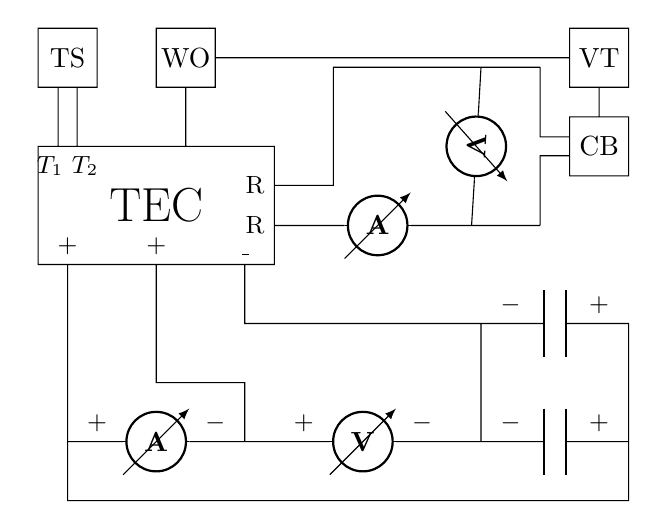
\begin{tikzpicture}[scale=1.5]
\draw
(0,0) rectangle (2,1)
(1,0.5) node{\LARGE TEC}
(4.5,0.75) rectangle (5,1.25)
(4.75,1) node{CB}
(4.75,1.25) -- (4.75,1.5)
(4.5,1.5) rectangle (5,2)
(4.75,1.75) node{VT}
(0,1.5) rectangle (0.5,2)
(0.25,1.75) node{TS}
(0.17,1) -- (0.17,1.5)
(0.33,1) -- (0.33,1.5)
(0.25,1) node[below]{\small $T_1~T_2$}
(4.5,0.92) -| (4.25,0.33)
(4.5,1.08) -| (4.25,1.67)
(2,0.33) to[ammeter] (3.75,0.33) -- (4.25,0.33)
(2,0.33) node[left]{\small R}
(4.25,1.67) -- (3.75,1.67) to[voltmeter] (3.67,0.33)
(3.75,1.67) -| (2.5,0.67) -- (2,0.67) node[left]{\small R}
(1,1.5) rectangle (1.5,2)
(1.25,1.75) node{WO}
(1.25,1.5) -- (1.25,1)
(1.5,1.75) -- (4.5,1.75)
(0.25,0) -- (0.25,-1.5) to[ammeter] (1.75,-1.5) to[voltmeter] (3.75,-1.5) to[capacitor] (5,-1.5)
(0.25,0) node[above]{\small +}
(3.75,-1.5) -- (3.75,-0.5) to[capacitor] (5,-0.5) -- (5,-1.5)
(3.75,-0.5) -| (1.75,0) node[above]{\small \_}
(1.75,-1.5) -- (1.75,-1) -| (1,0) node[above]{\small +}
(0.25,-1.5) |- (5,-2) -- (5,-1.5)
(0.5,-1.5) node[above]{\small +}
(1.5,-1.5) node[above]{\small $-$}
(2.25,-1.5) node[above]{\small +}
(3.25,-1.5) node[above]{\small $-$}
(4,-0.5) node[above]{\small $-$}
(4.75,-0.5) node[above]{\small +}
(4,-1.5) node[above]{\small $-$}
(4.75,-1.5) node[above]{\small +};
\end{tikzpicture}}
{The circuit used in the experiment.
The lower ammeter and voltmeter are set to DC.
The upper ammeter and voltmeter are set to AC.
TEC is the thermo-electric cooler.
TS is the temperature sensor.
WO is the wall outlet.
VT is the Variac transformer.
CB is the current balance.
The filter capacitors are shown on the bottom right.
The points $T_1$ and $T_2$ are the temperature of the heat sink, $T_\text{out}$, and the temperature of the reservoir, $T_\text{in}$, respectively.
The two positive ports and the negative port of the TEC are indicated with pluses and a minus, respectively.
The resistor ports of the TEC are indicated with the letter R.
Positive and negative terminals were not shown on the upper ammeter and voltmeter as they do not affect the results by more than a sign.}
	
\papersec{Observations}
	
	To begin with, the temperatures of the input and output reservoirs and the ambient air were measured for several values of input power. To make the measurements, the terminals were open-circuited (obtained by unplugging one of the chords connecting the TEC to the DC ammeter).
	
	The ambient temperature was determined to be \( \pars{22.1 \pm 0.1} \si{\celsius} \), and was found to remain constant throughout the obtaining of the measurements. 
	
	The following are measured values of the temperatures of the input reservoir, the heat sink, the input potential and the input current.
	
	\paperfig{TableOne}{\centering\begin{papertable}{|[outer]I|[inner]C|[inner]C|[inner]U|[inner]U|[outer]}\paperoline
			\papertableindexheader\papertablecheadersymbol{T_{out}}\papertablecheadersymbol{T_{in}}\papertableuheadersymbol{V_{in}}\papertableuheadersymbole{I_{in}}\\
			\papertablecheadersymbol{\pm.1\degree}\papertablecheadersymbol{\pm.1\degree}\papertableuheaderunit{\si{\volt}}\papertableuheaderunite{\si{\ampere}}\\\paperiline
			\papertableindex\papertablecval{23.0}\papertablecval{31.8}\papertableuval{3.197}{.005}\papertableuval{1.54}{.01}\\\paperiline
			\papertableindex\papertablecval{22.9}\papertablecval{31.4}\papertableuval{2.884}{.004}\papertableuval{1.39}{.01}\\\paperiline
			\papertableindex\papertablecval{22.9}\papertablecval{30.2}\papertableuval{2.488}{.004}\papertableuval{1.20}{.01}\\\paperiline
			\papertableindex\papertablecval{22.7}\papertablecval{27.4}\papertableuval{2.044}{.004}\papertableuval{0.98}{.01}\\\paperiline
			\papertableindex\papertablecval{22.5}\papertablecval{25.3}\papertableuval{1.441}{.004}\papertableuval{0.693}{.008}\\\paperiline
			\papertableindex\papertablecval{22.3}\papertablecval{23.3}\papertableuval{0.014}{.003}\papertableuval{0.006}{.005}\\\paperoline
	\end{papertable}\vspace{-0.5em}}{Measurements of $T_{out}$ ($\si{\celsius}$), $T_{in}$ ($\si{\celsius}$), $I_{in}$ ($\si{\ampere}$), and $V_{in}$ ($\si{\volt}$) for the first part of the experiment.}

	\bgroup\centering\begin{papertable}{|[outer]I|[inner]C|[inner]C|[inner]U|[inner]U|[outer]}\paperoline
	\papertableindexheader\papertablecheadersymbol{T_{out}}\papertablecheadersymbol{T_{in}}\papertableuheadersymbol{V_d}\papertableuheadersymbole{I_d}\\
	\papertablecheadersymbol{\pm.1\degree}\papertablecheadersymbol{\pm.1\degree}\papertableuheaderunit{\si{\volt}}\papertableuheaderunite{\si{\ampere}}\\\paperiline
\papertableindex\papertablecval{22.2}\papertablecval{20.6}\papertableuval{2.68}{.07}\papertableuval{9.77}{.03}\\\paperiline
\papertableindex\papertablecval{24.7}\papertablecval{16.7}\papertableuval{2.72}{.07}\papertableuval{9.73}{.03}\\\paperiline
\papertableindex\papertablecval{25.7}\papertablecval{15.0}\papertableuval{2.71}{.07}\papertableuval{9.47}{.02}\\\paperiline
\papertableindex\papertablecval{26.4}\papertablecval{13.4}\papertableuval{2.69}{.07}\papertableuval{9.49}{.02}\\\paperiline
\papertableindex\papertablecval{27.1}\papertablecval{11.3}\papertableuval{2.66}{.07}\papertableuval{9.29}{.02}\\\paperiline
\papertableindex\papertablecval{27.3}\papertablecval{10.4}\papertableuval{2.63}{.07}\papertableuval{9.21}{.02}\\\paperiline
\papertableindex\papertablecval{27.6}\papertablecval{9.1}\papertableuval{2.63}{.07}\papertableuval{9.17}{.02}\\\paperiline
\papertableindex\papertablecval{27.8}\papertablecval{8.0}\papertableuval{2.66}{.07}\papertableuval{9.22}{.02}\\\paperiline
\papertableindex\papertablecval{28.0}\papertablecval{6.8}\papertableuval{2.60}{.07}\papertableuval{9.01}{.02}\\\paperiline
\papertableindex\papertablecval{28.1}\papertablecval{5.9}\papertableuval{2.75}{.08}\papertableuval{9.57}{.02}\\\paperiline
\papertableindex\papertablecval{28.2}\papertablecval{4.8}\papertableuval{2.78}{.08}\papertableuval{9.65}{.03}\\\paperiline
\papertableindex\papertablecval{28.4}\papertablecval{4.0}\papertableuval{2.78}{.08}\papertableuval{9.63}{.03}\\\paperiline
\papertableindex\papertablecval{28.4}\papertablecval{3.1}\papertableuval{2.79}{.08}\papertableuval{9.65}{.03}\\\paperiline
\papertableindex\papertablecval{28.5}\papertablecval{2.3}\papertableuval{2.80}{.08}\papertableuval{9.67}{.03}\\\paperiline
\papertableindex\papertablecval{28.5}\papertablecval{1.5}\papertableuval{2.80}{.08}\papertableuval{9.68}{.03}\\\paperiline
\papertableindex\papertablecval{28.6}\papertablecval{0.7}\papertableuval{2.81}{.08}\papertableuval{9.70}{.03}\\\paperiline
\papertableindex\papertablecval{28.6}\papertablecval{0.1}\papertableuval{2.80}{.08}\papertableuval{9.68}{.03}\\\paperiline
\papertableindex\papertablecval{28.6}\papertablecval{-0.4}\papertableuval{2.80}{.08}\papertableuval{9.68}{.03}\\\paperiline
\papertableindex\papertablecval{28.6}\papertablecval{-1.1}\papertableuval{2.82}{.08}\papertableuval{9.71}{.03}\\\paperiline
\papertableindex\papertablecval{28.6}\papertablecval{-1.7}\papertableuval{2.82}{.08}\papertableuval{9.71}{.03}\\\paperiline
\papertableindex\papertablecval{28.6}\papertablecval{-2.7}\papertableuval{2.81}{.08}\papertableuval{9.69}{.03}\\\paperiline
\papertableindex\papertablecval{28.6}\papertablecval{-3.3}\papertableuval{2.83}{.08}\papertableuval{9.74}{.03}\\\paperiline
\papertableindex\papertablecval{28.6}\papertablecval{-3.7}\papertableuval{2.81}{.08}\papertableuval{9.68}{.03}\\\paperiline
\papertableindex\papertablecval{28.6}\papertablecval{-4.2}\papertableuval{2.81}{.08}\papertableuval{9.67}{.03}\\\paperiline
\papertableindex\papertablecval{28.5}\papertablecval{-4.7}\papertableuval{2.74}{.07}\papertableuval{9.42}{.02}\\\paperiline
\papertableindex\papertablecval{28.3}\papertablecval{-5.2}\papertableuval{2.73}{.07}\papertableuval{9.35}{.02}\\\paperiline
\papertableindex\papertablecval{28.2}\papertablecval{-5.5}\papertableuval{2.70}{.07}\papertableuval{9.28}{.02}\\\paperiline
\papertableindex\papertablecval{28.2}\papertablecval{-5.7}\papertableuval{2.71}{.07}\papertableuval{9.30}{.02}\\\paperoline\end{papertable}\egroup

\paperfig{PartTwoA}{\centering\begin{papertable}{|[outer]I|[inner]C|[inner]C|[inner]U|[inner]U|[outer]}\paperoline
	\papertableindexheader\papertablecheadersymbol{T_{out}}\papertablecheadersymbol{T_{in}}\papertableuheadersymbol{V_d}\papertableuheadersymbole{I_d}\\
	\papertablecheadersymbol{\pm.1\degree}\papertablecheadersymbol{\pm.1\degree}\papertableuheaderunit{\si{\volt}}\papertableuheaderunite{\si{\ampere}}\\\paperiline
\stepcounter{papertableindexcounter}\stepcounter{papertableindexcounter}\stepcounter{papertableindexcounter}\stepcounter{papertableindexcounter}\stepcounter{papertableindexcounter}\stepcounter{papertableindexcounter}\stepcounter{papertableindexcounter}\stepcounter{papertableindexcounter}\stepcounter{papertableindexcounter}\stepcounter{papertableindexcounter}\stepcounter{papertableindexcounter}\stepcounter{papertableindexcounter}\stepcounter{papertableindexcounter}\stepcounter{papertableindexcounter}\stepcounter{papertableindexcounter}\stepcounter{papertableindexcounter}\stepcounter{papertableindexcounter}\stepcounter{papertableindexcounter}\stepcounter{papertableindexcounter}\stepcounter{papertableindexcounter}\stepcounter{papertableindexcounter}\stepcounter{papertableindexcounter}\stepcounter{papertableindexcounter}\stepcounter{papertableindexcounter}\stepcounter{papertableindexcounter}\stepcounter{papertableindexcounter}\stepcounter{papertableindexcounter}\stepcounter{papertableindexcounter}\papertableindex\papertablecval{28.1}\papertablecval{-5.9}\papertableuval{2.71}{.07}\papertableuval{9.33}{.02}\\\paperiline
\papertableindex\papertablecval{28.1}\papertablecval{-6.2}\papertableuval{2.64}{.07}\papertableuval{9.22}{.02}\\\paperiline
\papertableindex\papertablecval{28.1}\papertablecval{-6.3}\papertableuval{2.67}{.07}\papertableuval{9.21}{.02}\\\paperiline
\papertableindex\papertablecval{28.0}\papertablecval{-6.5}\papertableuval{2.68}{.07}\papertableuval{9.21}{.02}\\\paperiline
\papertableindex\papertablecval{28.0}\papertablecval{-6.7}\papertableuval{2.72}{.07}\papertableuval{9.34}{.02}\\\paperiline
\papertableindex\papertablecval{27.9}\papertablecval{-6.9}\papertableuval{2.80}{.08}\papertableuval{9.72}{.03}\\\paperiline
\papertableindex\papertablecval{27.9}\papertablecval{-7.1}\papertableuval{2.67}{.07}\papertableuval{9.21}{.02}\\\paperiline
\papertableindex\papertablecval{27.9}\papertablecval{-7.2}\papertableuval{2.65}{.07}\papertableuval{9.16}{.02}\\\paperiline
\papertableindex\papertablecval{27.9}\papertablecval{-7.4}\papertableuval{2.64}{.07}\papertableuval{9.15}{.02}\\\paperiline
\papertableindex\papertablecval{27.8}\papertablecval{-7.4}\papertableuval{2.85}{.08}\papertableuval{9.98}{.03}\\\paperiline
\papertableindex\papertablecval{27.9}\papertablecval{-7.6}\papertableuval{2.87}{.08}\papertableuval{10.06}{.03}\\\paperiline
\papertableindex\papertablecval{28.1}\papertablecval{-7.9}\papertableuval{2.87}{.08}\papertableuval{10.05}{.03}\\\paperiline
\papertableindex\papertablecval{28.1}\papertablecval{-8.1}\papertableuval{2.87}{.08}\papertableuval{10.08}{.03}\\\paperiline
\papertableindex\papertablecval{28.2}\papertablecval{-8.2}\papertableuval{2.85}{.08}\papertableuval{10.00}{.03}\\\paperiline
\papertableindex\papertablecval{28.3}\papertablecval{-8.3}\papertableuval{2.87}{.08}\papertableuval{10.13}{.03}\\\paperiline
\papertableindex\papertablecval{28.3}\papertablecval{-8.5}\papertableuval{2.88}{.08}\papertableuval{10.14}{.03}\\\paperiline
\papertableindex\papertablecval{28.3}\papertablecval{-8.6}\papertableuval{2.87}{.08}\papertableuval{10.16}{.03}\\\paperiline
\papertableindex\papertablecval{28.3}\papertablecval{-8.7}\papertableuval{2.88}{.08}\papertableuval{10.22}{.03}\\\paperiline
\papertableindex\papertablecval{28.3}\papertablecval{-8.7}\papertableuval{2.88}{.08}\papertableuval{10.22}{.03}\\\paperiline
\papertableindex\papertablecval{28.3}\papertablecval{-8.6}\papertableuval{2.85}{.08}\papertableuval{10.09}{.03}\\\paperiline
\papertableindex\papertablecval{28.3}\papertablecval{-8.8}\papertableuval{2.72}{.07}\papertableuval{9.70}{.03}\\\paperiline
\papertableindex\papertablecval{28.3}\papertablecval{-8.9}\papertableuval{2.76}{.08}\papertableuval{9.79}{.03}\\\paperiline
\papertableindex\papertablecval{28.2}\papertablecval{-8.9}\papertableuval{2.72}{.07}\papertableuval{9.66}{.03}\\\paperiline
\papertableindex\papertablecval{28.1}\papertablecval{-8.9}\papertableuval{2.84}{.08}\papertableuval{10.17}{.03}\\\paperiline
\papertableindex\papertablecval{28.1}\papertablecval{-8.9}\papertableuval{2.84}{.08}\papertableuval{10.20}{.03}\\\paperiline
\papertableindex\papertablecval{28.1}\papertablecval{-9.0}\papertableuval{2.85}{.08}\papertableuval{10.25}{.03}\\\paperiline
\papertableindex\papertablecval{28.1}\papertablecval{-9.0}\papertableuval{2.85}{.08}\papertableuval{10.27}{.03}\\\paperiline
\papertableindex\papertablecval{28.2}\papertablecval{-9.1}\papertableuval{2.85}{.08}\papertableuval{10.31}{.03}\\\paperoline
\end{papertable}\vspace{-0.5em}}{Measurements of $T_{out}$ ($\si{\celsius}$), $T_{in}$ ($\si{\celsius}$), $V_d$ ($\si{\volt}$), and $I_d$ ($\si{\ampere}$) for the first part of the second part of the experiment.}

	Further, after allowing the system to cool off, the TEC was operated with an approximately fixed current supplied from the built-in power supply. The Variac transformer was turned off; measurements of voltage across the TEC and the current supplied to it, as well as the temperatures of the output and the input reservoir were taken (see \figPartTwoA).
	
	One of the main sources of error in the experiment was the non-constant potential of the current balance, which seemed to always be smaller than the marked potential of 6 volts. For this reason, a fourth multimeter was used in the data collection to account for this.

	\paperfig{TableTwoBOne}{\centering\begin{papertable}{|[outer]I|[inner]C|[inner]C|[inner]C|[inner]C|[outer]}\paperoline
			\papertableindexheader\papertablecheadersymbol{T_{out}}\papertablecheadersymbol{T_{in}}\papertablecheadersymbol{V_d~(\si{\volt})}\papertablecheadersymbol{I_d~(\si{\ampere})}\\
			\papertablecheadersymbol{\pm.1\degree}\papertablecheadersymbol{\pm.1\degree}\papertablecheaderunit{.004}{$\si{\volt}$}\papertablecheaderunit{.3}{$\si{\ampere}$}\\\paperiline
\papertableindex\papertablecval{27.9}\papertablecval{-7.0}\papertablecval{2.573}\papertablecval{12.1}\\\paperiline
\papertableindex\papertablecval{27.9}\papertablecval{-6.6}\papertablecval{2.603}\papertablecval{12.6}\\\paperiline
\papertableindex\papertablecval{28.0}\papertablecval{-5.3}\papertablecval{2.524}\papertablecval{12.4}\\\paperiline
\papertableindex\papertablecval{28.0}\papertablecval{-3.9}\papertablecval{2.535}\papertablecval{12.8}\\\paperiline
\papertableindex\papertablecval{28.0}\papertablecval{-2.7}\papertablecval{2.510}\papertablecval{12.8}\\\paperiline
\papertableindex\papertablecval{28.1}\papertablecval{-1.4}\papertablecval{2.479}\papertablecval{12.9}\\\paperiline
\papertableindex\papertablecval{28.9}\papertablecval{-0.3}\papertablecval{2.752}\papertablecval{14.8}\\\paperiline
\papertableindex\papertablecval{29.4}\papertablecval{0.4}\papertablecval{2.742}\papertablecval{15.0}\\\paperiline
\papertableindex\papertablecval{28.9}\papertablecval{2.2}\papertablecval{2.447}\papertablecval{13.6}\\\paperiline
\papertableindex\papertablecval{28.5}\papertablecval{4.0}\papertablecval{2.512}\papertablecval{14.3}\\\paperiline
\papertableindex\papertablecval{28.7}\papertablecval{5.4}\papertablecval{2.542}\papertablecval{14.8}\\\paperoline
	\end{papertable}\vspace{-0.5em}}{Measurements of $T_{out}$ ($\si{\celsius}$), $T_d$ ($\si{\celsius}$), $V_d$ ($\si{\volt}$), and $I_d$ ($\si{\ampere}$) for the second part of the second part of the experiment.}\vspace{2em}

	\paperfig{TableTwoBTwo}{\centering\begin{papertable}{|[outer]I|[inner]U|[inner]U|[inner]C|[outer]}\paperoline
			\papertableindexheader\papertableuheadersymbol{V_{in}}\papertableuheadersymbol{I_{in}}\papertablecheadersymbol{V_s}\\
			\papertableuheadersymbol{(\si{\volt})}\papertableuheadersymbol{(\si{\ampere})}\papertablecheadersymbol{(\si{\volt})}\\\paperiline
\papertableindex\papertableuval{0.00}{.02}\papertableuval{0.00}{.01}\papertablecval{0.408}\\\paperiline
\papertableindex\papertableuval{0.67}{.03}\papertableuval{1.50}{.05}\papertablecval{0.396}\\\paperiline
\papertableindex\papertableuval{0.95}{.04}\papertableuval{2.12}{.06}\papertablecval{0.392}\\\paperiline
\papertableindex\papertableuval{1.16}{.04}\papertableuval{2.57}{.07}\papertablecval{0.367}\\\paperiline
\papertableindex\papertableuval{1.34}{.05}\papertableuval{2.99}{.08}\papertablecval{0.353}\\\paperiline
\papertableindex\papertableuval{1.50}{.05}\papertableuval{3.33}{.09}\papertablecval{0.336}\\\paperiline
\papertableindex\papertableuval{1.66}{.05}\papertableuval{3.6}{.1}\papertablecval{0.339}\\\paperiline
\papertableindex\papertableuval{1.78}{.06}\papertableuval{3.9}{.1}\papertablecval{0.337}\\\paperiline
\papertableindex\papertableuval{1.90}{.06}\papertableuval{4.2}{.1}\papertablecval{0.304}\\\paperiline
\papertableindex\papertableuval{2.03}{.06}\papertableuval{4.4}{.1}\papertablecval{0.281}\\\paperiline
\papertableindex\papertableuval{2.13}{.06}\papertableuval{4.7}{.1}\papertablecval{0.273}\\\paperoline
	\end{papertable}\vspace{-0.5em}}{Measurements of $V_{in}$ ($\si{\volt}$), $I_{in}$ ($\si{\ampere}$), and $V_s$ ($\si{\volt}$) for the second part of the second part of the experiment.}\vspace{2em}


	Finally, after reaching a \( 30 \si{\celsius} \) temperature difference, the Variac transformer was turned on to supply various power inputs to the system. Allowing the system to reach a semi-stable state (waiting roughly two minutes after changing the power), reservoir temperatures, input and output power, and the Seebeck voltage were measured. The Seebeck voltage was obtained by turning off the TEC and recording the highest reading of continuously running-off potential. 

\papersec{Analysis} 
	
	To visualize the data with the open-circuited terminals, temperature difference was plotted against the input power. Uncertainties were propagated using the method of quadratures.\\
	
	\paperfig{PartOne}{\pdf{1}}{Temperature difference plotted against the power for the open-circuited terminals. The error bars were included but were too small to be visible. Linear functions were fitted to the two curves in the graph. The reciprocals of their slopes are the thermal conductances between the relevant materials. The thermal conductance between the two reservoirs, $K_d$, was found to be $(0.59\pm.06)\si{\watt\per\kelvin}$. This fit had a reduced $\chi^2$ of 24.2124 and an $R^2$ value of 0.962248. The thermal conductance between the output heat sink and the ambient, $K_{hs}$, air was found to be $(7.1\pm.9)\si{\watt\per\kelvin}$. This fit had a reduced $\chi^2$ of 0.307025 and an $R^2$ value of 0.933316. Residuals for the fits are shown below the plot.}\vspace{2em}
	
	To visualize the results for the fixed current setup supplied by the built-in power supply, temperature difference and the electrical power input were plotted against time. All uncertainties were propagates using the method of quadratures.
	
	The thermal conductance between the input and the output reservoirs, $K_d$, obeys the following relation.
	
	\papereq{Kd}{P_K=K_d\Delta T}{AF, 2014}
	\begin{paperwhere}
	\papervar{P_K}{power}{\watt}
	\papervar{K_d}{thermal conductance}{\watt\per\kelvin}
	\papervar{\Delta T}{temperature difference}{\kelvin}
	\end{paperwhere}

	The thermal conductance between the output heat sink and the ambient air, $K_{hs}$, obeys a similar relation. Thus, the values of $K_d$ and $K_{hs}$ were computed by fitting linear functions to the curves in \figPartOne and taking the reciprocals of the obtained values. The thermal conductance between the two reservoirs, $K_d$, was found to be $(0.59\pm.06)\si{\watt\per\kelvin}$.
The thermal conductance between the output heat sink and the ambient, $K_{hs}$, air was found to be $(7.1\pm.9)\si{\watt\per\kelvin}$.
	
	\paperfig{partTwoa}{\pdf{part2a-data}}{Power and temperature difference plotted against time. Uncertainties were included but were too small to be visible. An increasing exponential function with a plateau was fit to the temperature difference. The plateau was determined to have a height of $(37.3\pm.2)\si{\kelvin}$. This fit had a reduced $\chi^2$ of 20.3006 and an $R^2$ value of 0.994558. Residuals for the fit are shown below the plot.}
	
	An overall linear increase in the power input as a function of time was observed except for the rapid decreases that could be attributed to noise in the circuit.
	
	The TEC model was used to predict the lowest achievable temperature with no heat input. This was done by modeling the graph in \figpartTwoa as an increasing exponential function with a plateau. This resulted in the largest possible temperature difference, which was compared against the existing data in \figPartTwoA. As a result, the lowest achievable temperature at the thermal reservoir with no heat input was determined to be $(-9.1\pm.2)\si{\kelvin}$.
	
	To visualize the results for various power inputs supplied by the Variac transformer, reservoir temperatures, power, and the Seebeck voltage were plotted versus the input power. All uncertainties were propagates using the method of quadratures.
	
	\paperfig{part2b}{\pdf{part2b-data}}{Temperature vs. input power (left), total electrical power vs. input power (middle) and total voltage across the TEC vs. input power (right). Uncertainties were included but were too small to be visible.}\vspace{2em}
		
	The internal resistance of the thermoelectric cooler, $R_d$, was determined using Ohm's law.
	
	\papereq{OhmAgain}{R_d=\frac{V_d}{I_d}}{AF, 2014}
	\begin{paperwhere}
	\papervar{R_d}{TEC resistance}{\ohm}
	\papervar{V_d}{TEC potential}{\volt}
	\papervar{I_d}{TEC current}{\ampere}
	\end{paperwhere}
	
	By combining \eqOhmAgain with data from \figTableTwoBOne, the internal resistance of the thermoelectric cooler, $R_d$, was determined to be $(0.19\pm.01)\si{\ohm}$.
	
	By a similar process, the Seebeck coefficient was determined by using the model for the TEC.
	
	\papereq{Seebeck}{S_d=\frac{V_s}{\Delta T}}{AF, 2014}
	\begin{paperwhere}
	\papervar{S_d}{Seebeck coefficient}{\volt\per\kelvin}
	\papervar{V_s}{Seebeck potential}{\volt}
	\papervar{\Delta T}{temperature difference}{\kelvin}
	\end{paperwhere}
	
	By combining \eqSeebeck with data from \figTableTwoBOne and \figTableTwoBTwo, the Seebeck coefficient for the system, $S_d$, was determined to be $(11.6\pm.1)\si{\milli\volt\per\kelvin}$.
	
	By examining the derivative of $P_{in}$ with an output temperature of $\SI{35}{\celsius}$ and an input temperature not exceeding $\SI{5}{\celsius}$, the optimum input current was determined using the TEC model. It is known that $P_{in}$ obeys the following relation.\columnbreak
	
	\papereq{Pin}{\fontsize{10pt}{10pt}\selectfont P_{in}=(T_{out}-\Delta T)S_dI_d-\frac12R_dI^2_d-K_d\Delta T}{AF, 2014}
	\begin{paperwhere}
	\papervar{P_{in}}{input power}{\watt}
	\papervar{T_{out}}{output temperature}{\kelvin}
	\papervar{\Delta T}{temperature difference}{\kelvin}
	\papervar{S_d}{Seebeck coefficient}{\volt\per\kelvin}
	\papervar{I_d}{TEC current}{\ampere}
	\papervar{R_d}{TEC resistance}{\ohm}
	\papervar{K_d}{thermal conductance}{\watt\per\kelvin}
	\end{paperwhere}
	
	When differentiated and set to zero to find the maximum, the optimal input current was shown to be equal to the following.
	
	\papereq{Diff}{I_d=\frac{(T_{out}-\Delta T)S_d}{R_d}}{}
	\begin{paperwhere}
	\papervar{T_{out}}{output temperature}{\kelvin}
	\papervar{\Delta T}{temperature difference}{\kelvin}
	\papervar{S_d}{Seebeck coefficient}{\volt\per\kelvin}
	\papervar{I_d}{TEC current}{\ampere}
	\papervar{R_d}{TEC resistance}{\ohm}
	\end{paperwhere}
	
	The optimal current was thus found to be $(17.0\pm.9)\si{\ampere}$.
	
	If no heat were admitted to the reservoir, $P_{in}$ is set to 0. By using the value for the optimal current and rearranging \eqPin to solve for $T_{in}$, the lowest input temperature was shown to be $(-18.4\pm.3)\si{\celsius}$.
	
	Lastly, to have a dynamic model, the PID stabilization algorithm could be used. This could be done in combination with the well known heat equation to create a model for the spread of heat through the system. These partial differential equations could be solved with numerical methods for modeling the transition of heat between the boundaries of the TEC elements.
	
\papersec{Conclusion}

	Although most of the values obtained in this experiment had high precision, the experiment was not free from sources of error. The primary source of error was the fluctuating potential of the current balance. An attempt was made to mitigate this by adding a fourth multimeter to the data collection.

	A secondary source of error came from the fact that both the input thermal reservoir and the heat sink were both in contact with the surrounding air, in which eddies and other current were free to exchange heat, thereby introducing uncertainty into the measurements in this experiment.
	
	Aside from the sources of error, the experiment was successful in determining the key values in question. These were determined to be the following.
The thermal conductance between the two reservoirs, $K_d$, was found to be $(0.59\pm.06)\si{\watt\per\kelvin}$.
The thermal conductance between the output heat sink and the ambient, $K_{hs}$, air was found to be $(7.1\pm.9)\si{\watt\per\kelvin}$.
The Seebeck coefficient for the system, $S_d$, was determined to be $(11.6\pm.1)\si{\milli\volt\per\kelvin}$.
The internal resistance of the thermoelectric cooler, $R_d$, was determined to be $(0.19\pm.01)\si{\ohm}$.
The lowest achievable temperature at the thermal reservoir with no heat input was determined to be $(-9.1\pm.2)\si{\kelvin}$.
The optimum drive current for the system was determined to be $(17.0\pm.9)\si{\ampere}$.
The lowest achievable temperature with the optimum input current was determined to be $(-18.4\pm.3)\si{\celsius}$.

\papersec{Sources}

	\papersource{Albanelli, P., Fomichev, S., Thermoelectricity, 2014}

\end{paper}
\end{document}